\section{Results}

\begin{figure}
    \centering
    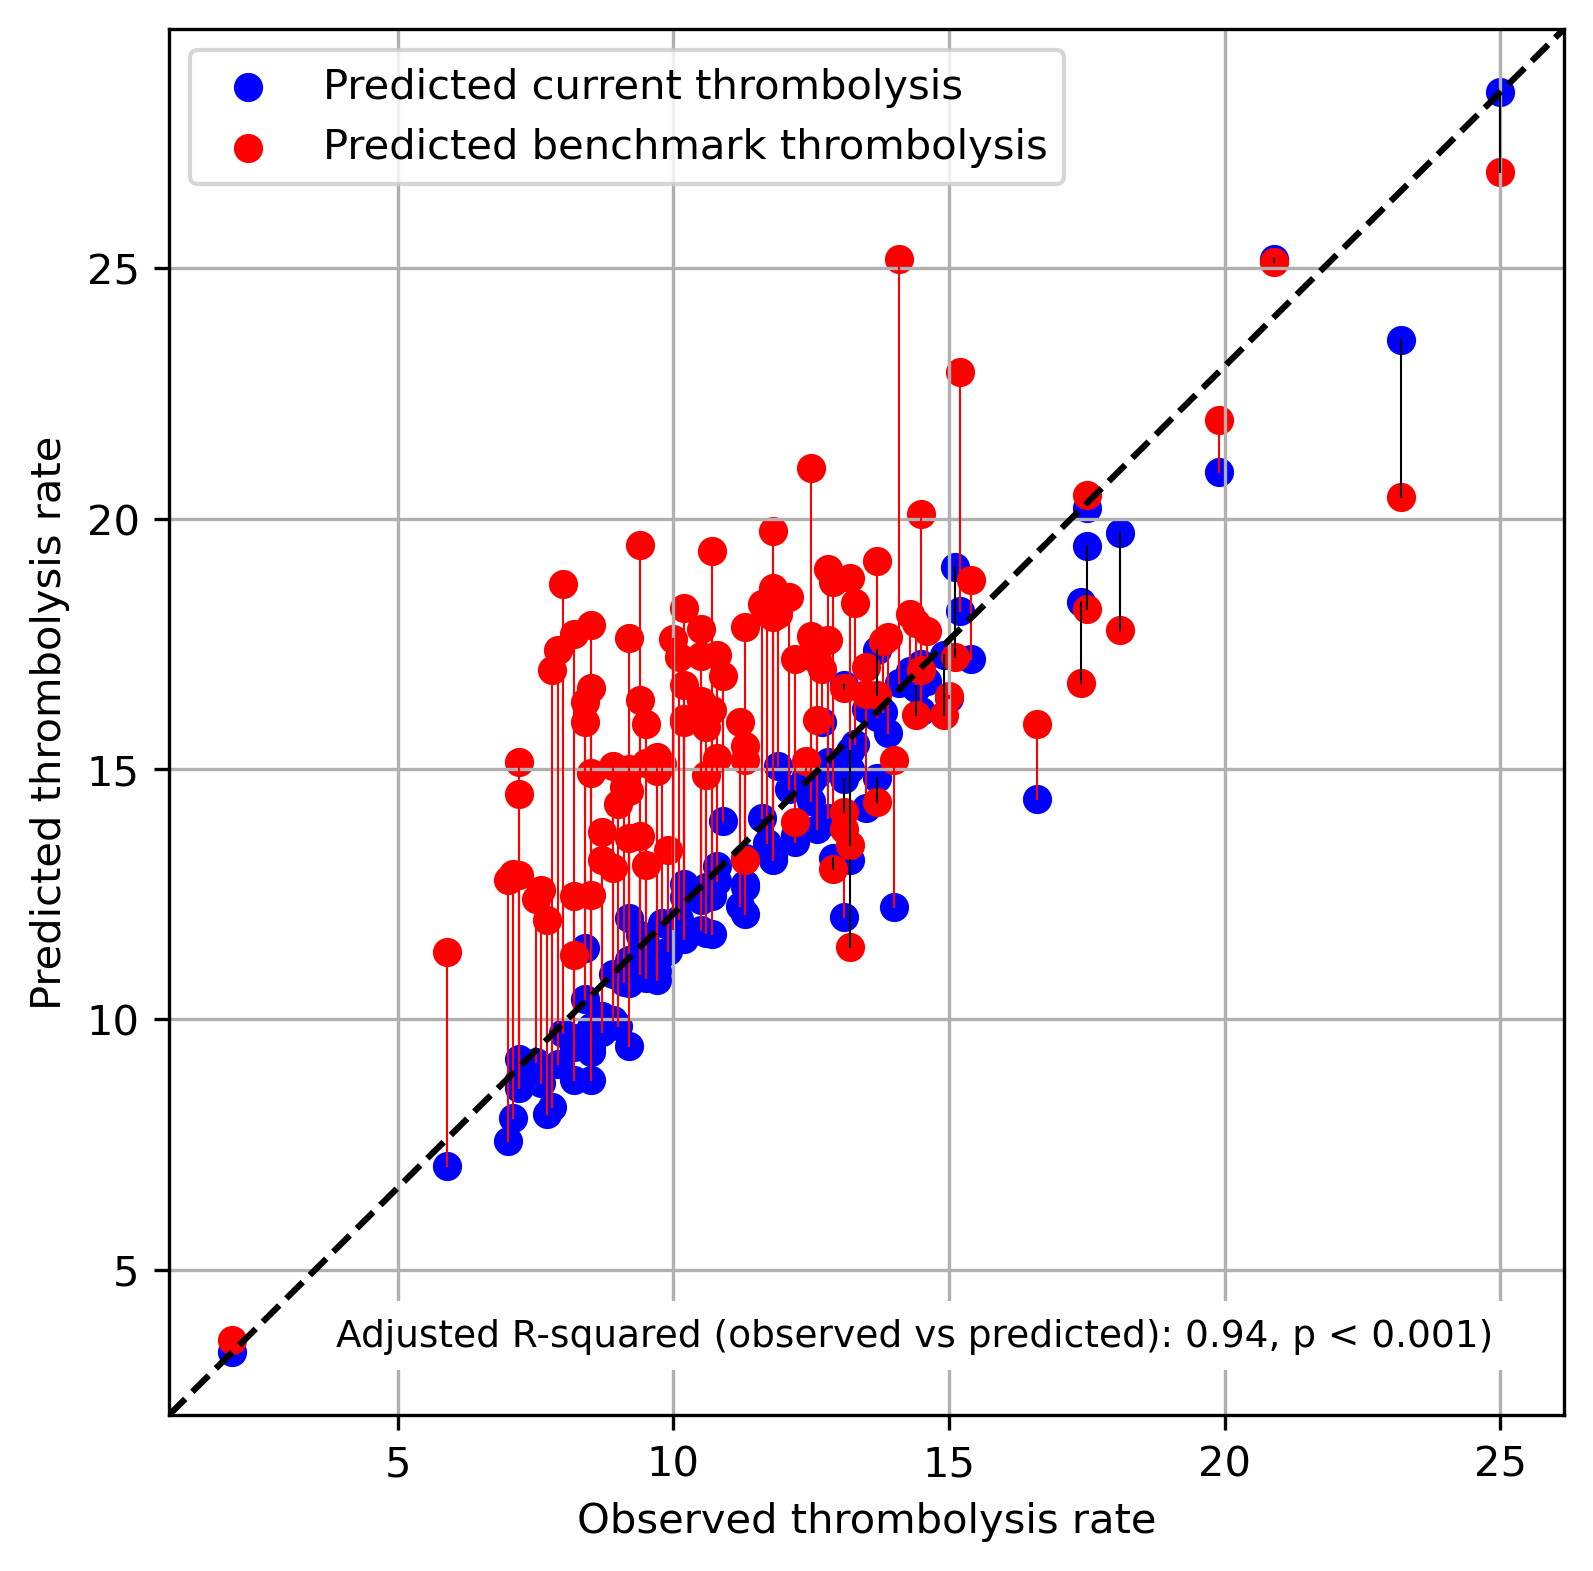
\includegraphics[width=0.65\linewidth]{images/thrombolysis_rates_model}
    \caption{Enter Caption}
    \label{fig:model_validation}
\end{figure}


\begin{figure}
    \centering
    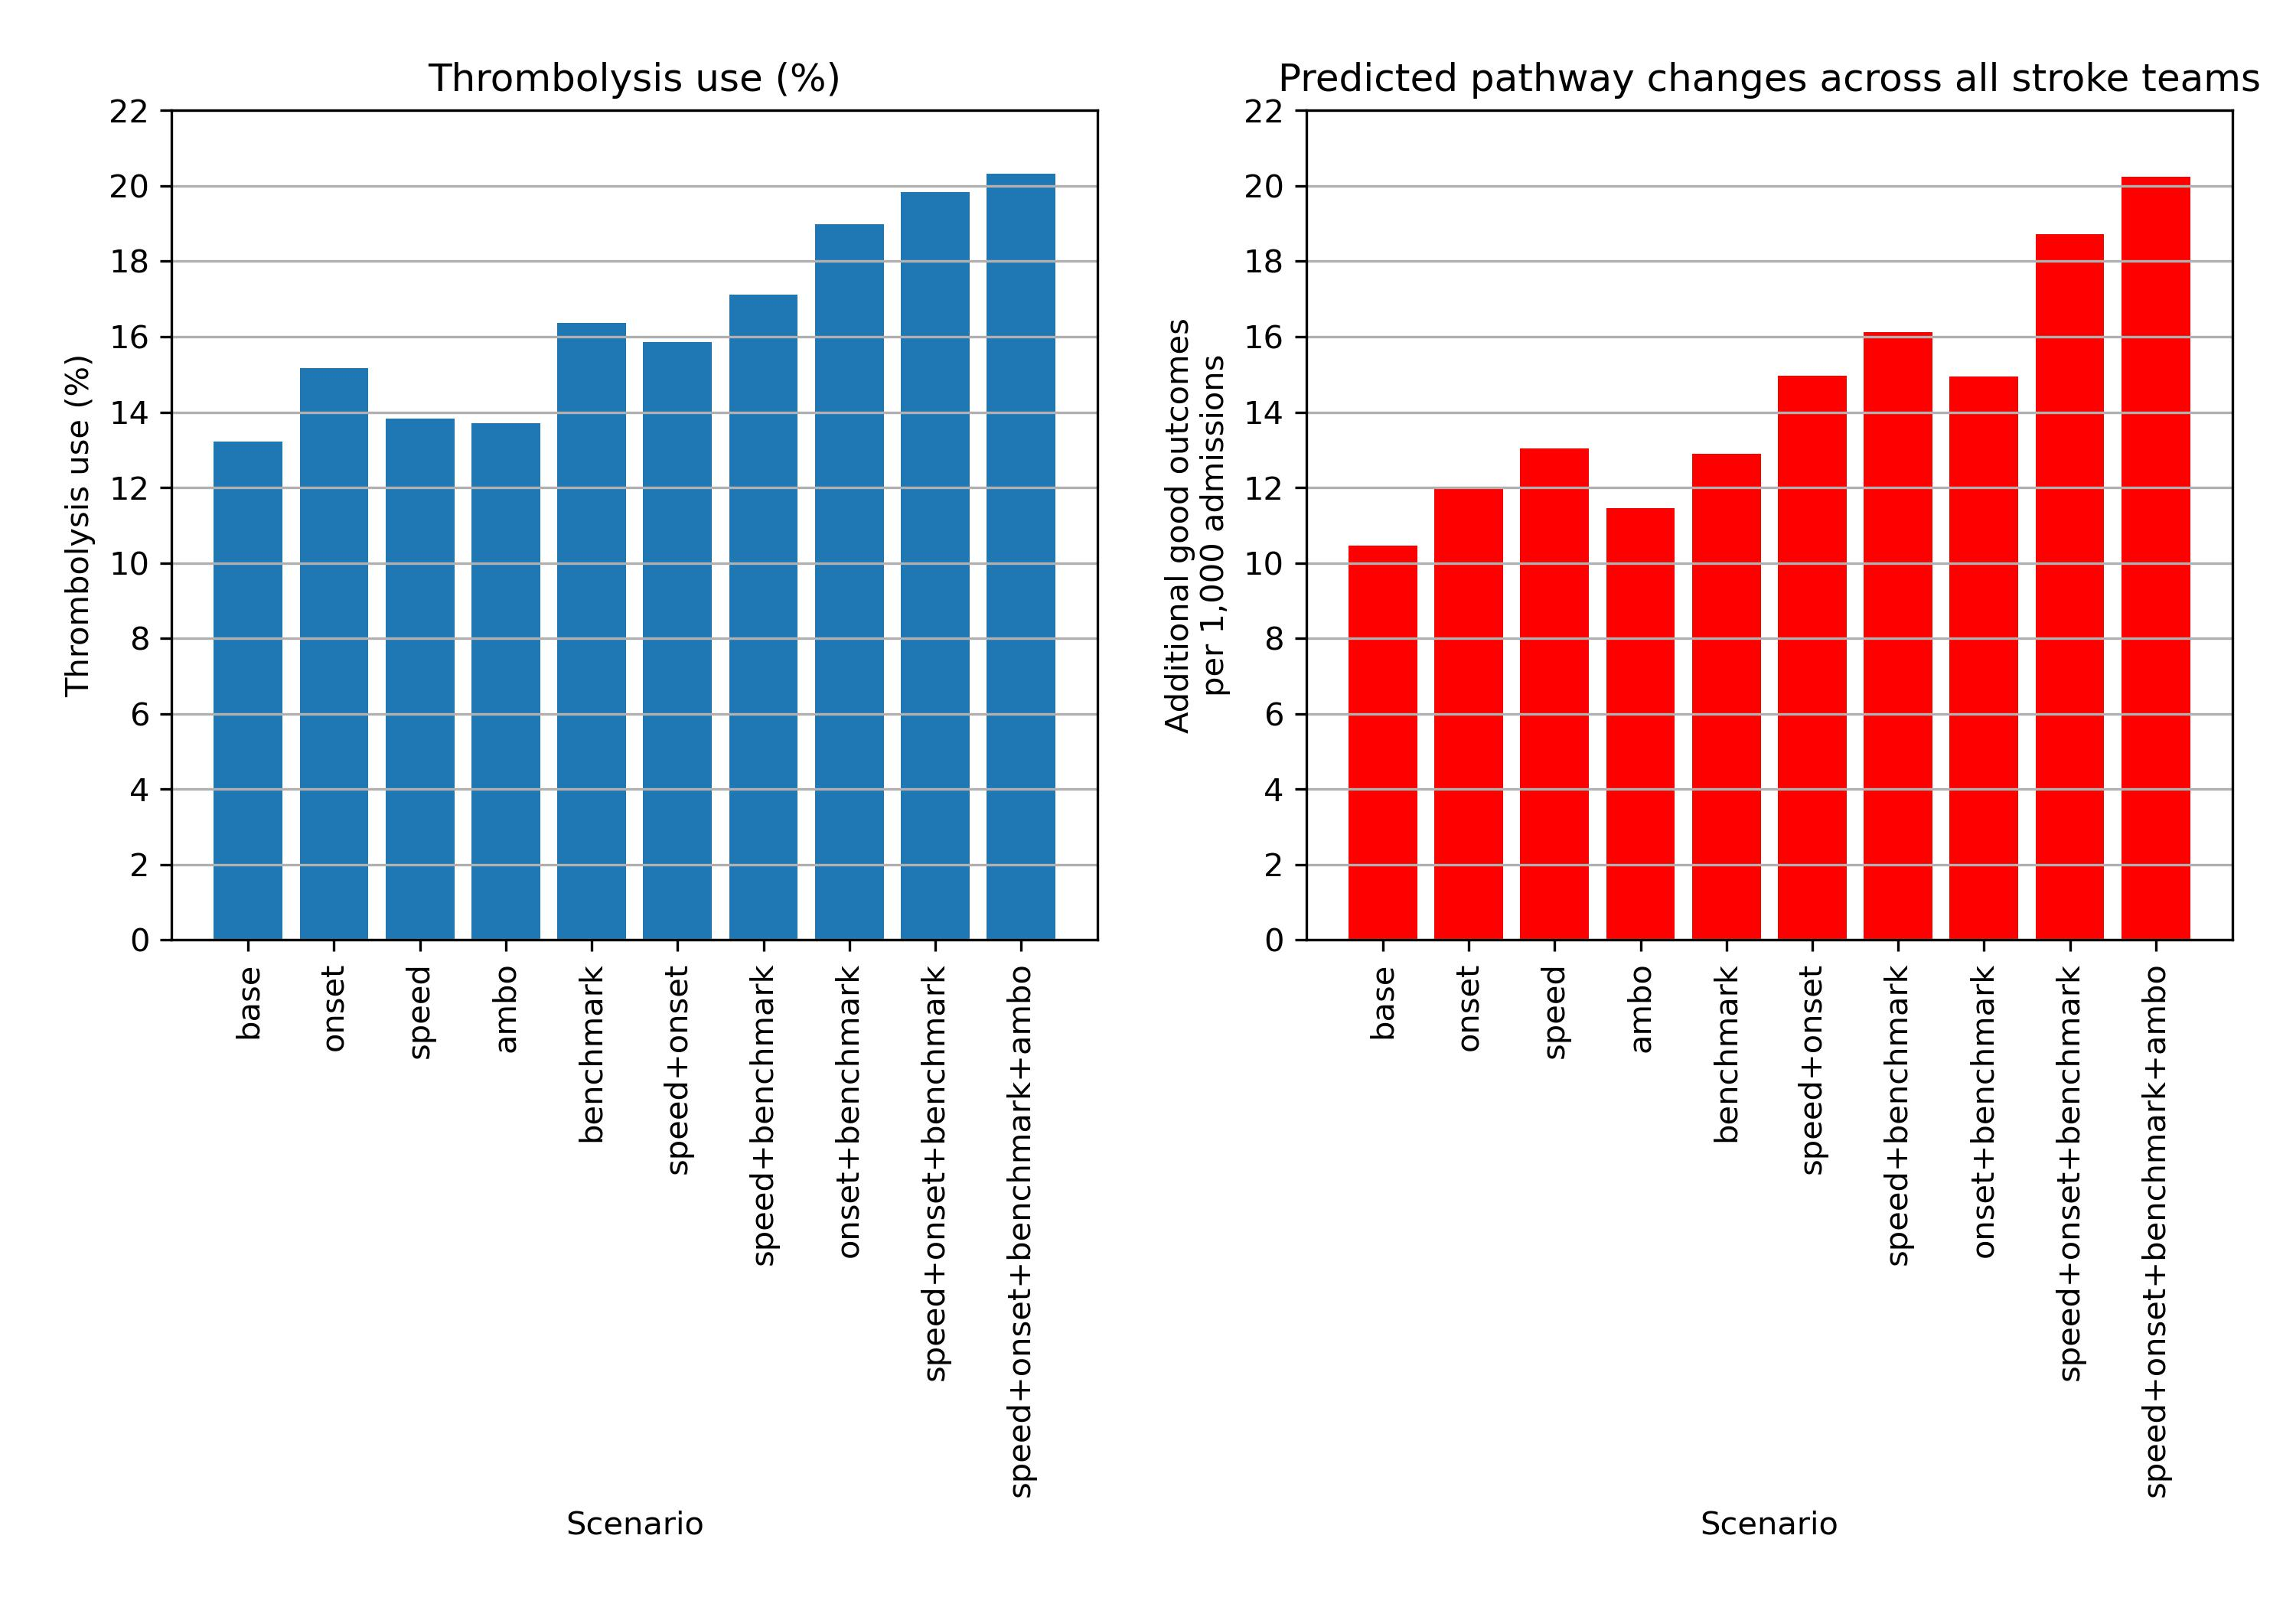
\includegraphics[width=0.75\linewidth]{images/sim_results_summary}
    \caption{Enter Caption}
    \label{fig:sim_results_summary}
\end{figure}

\begin{figure}
    \centering
    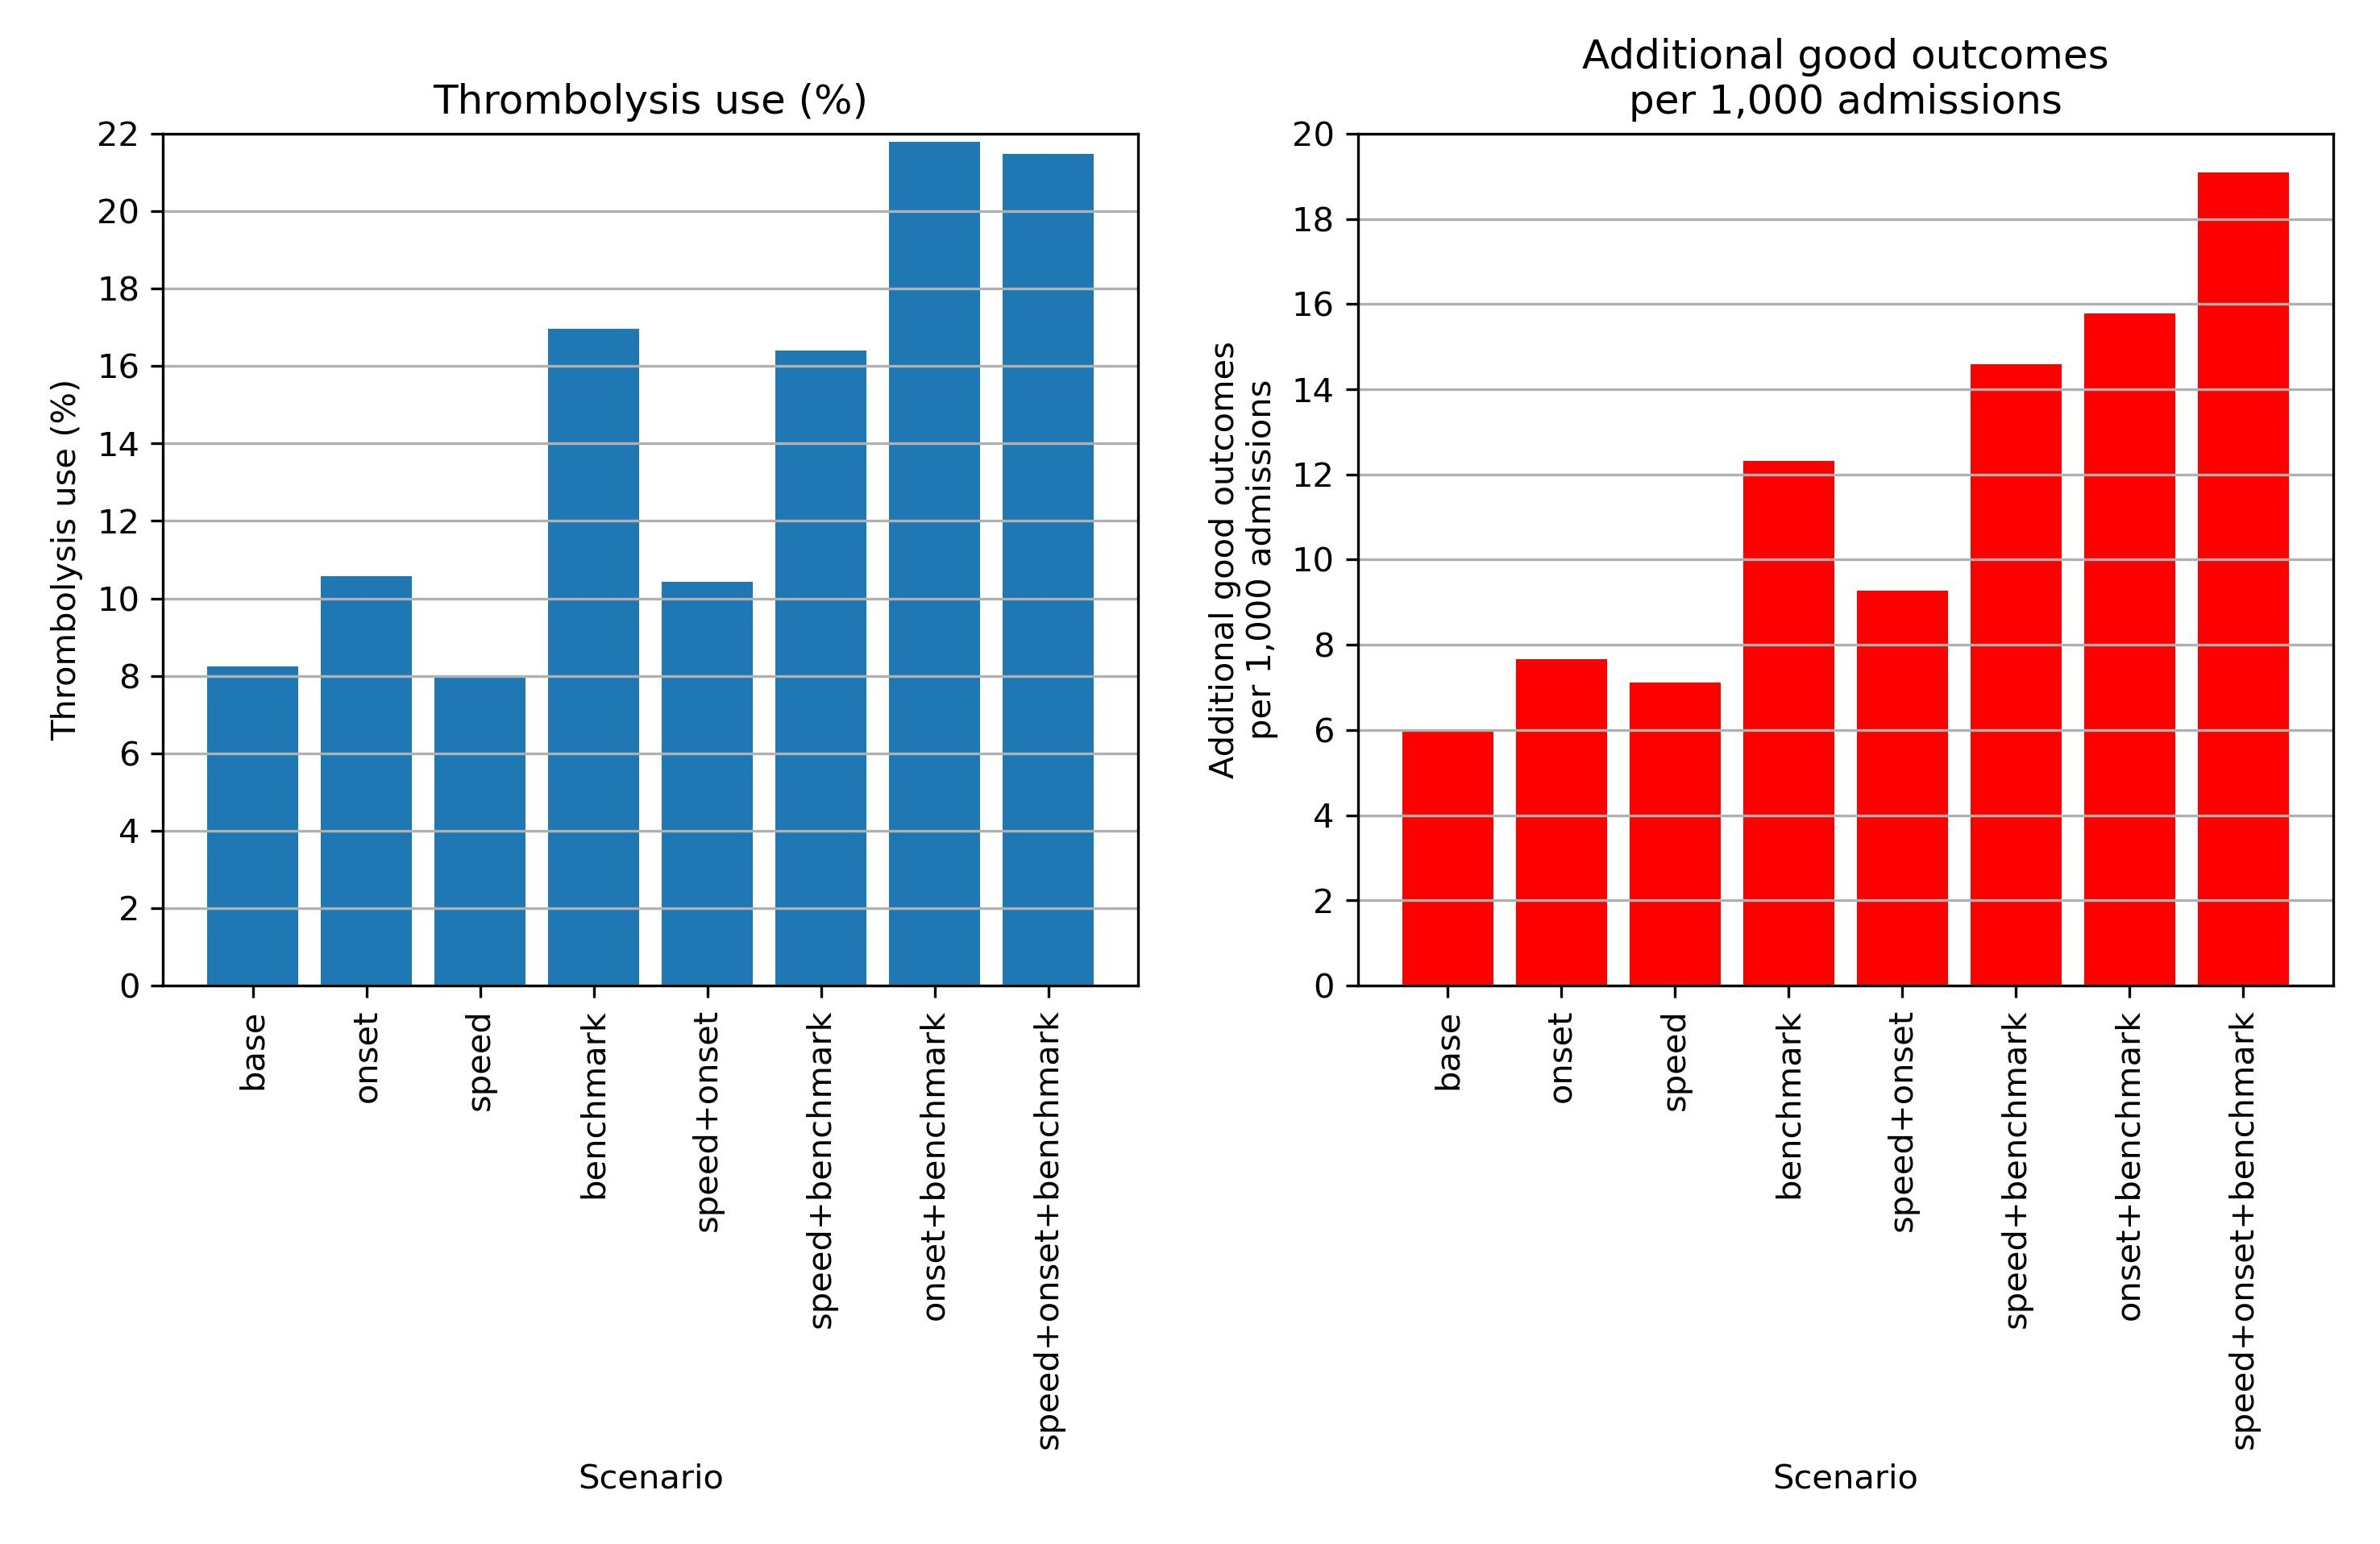
\includegraphics[width=0.75\linewidth]{images/sim_results_team_x}
    \caption{Enter Caption}
    \label{fig:sim_results_team_x}
\end{figure}

\begin{figure}
    \centering
    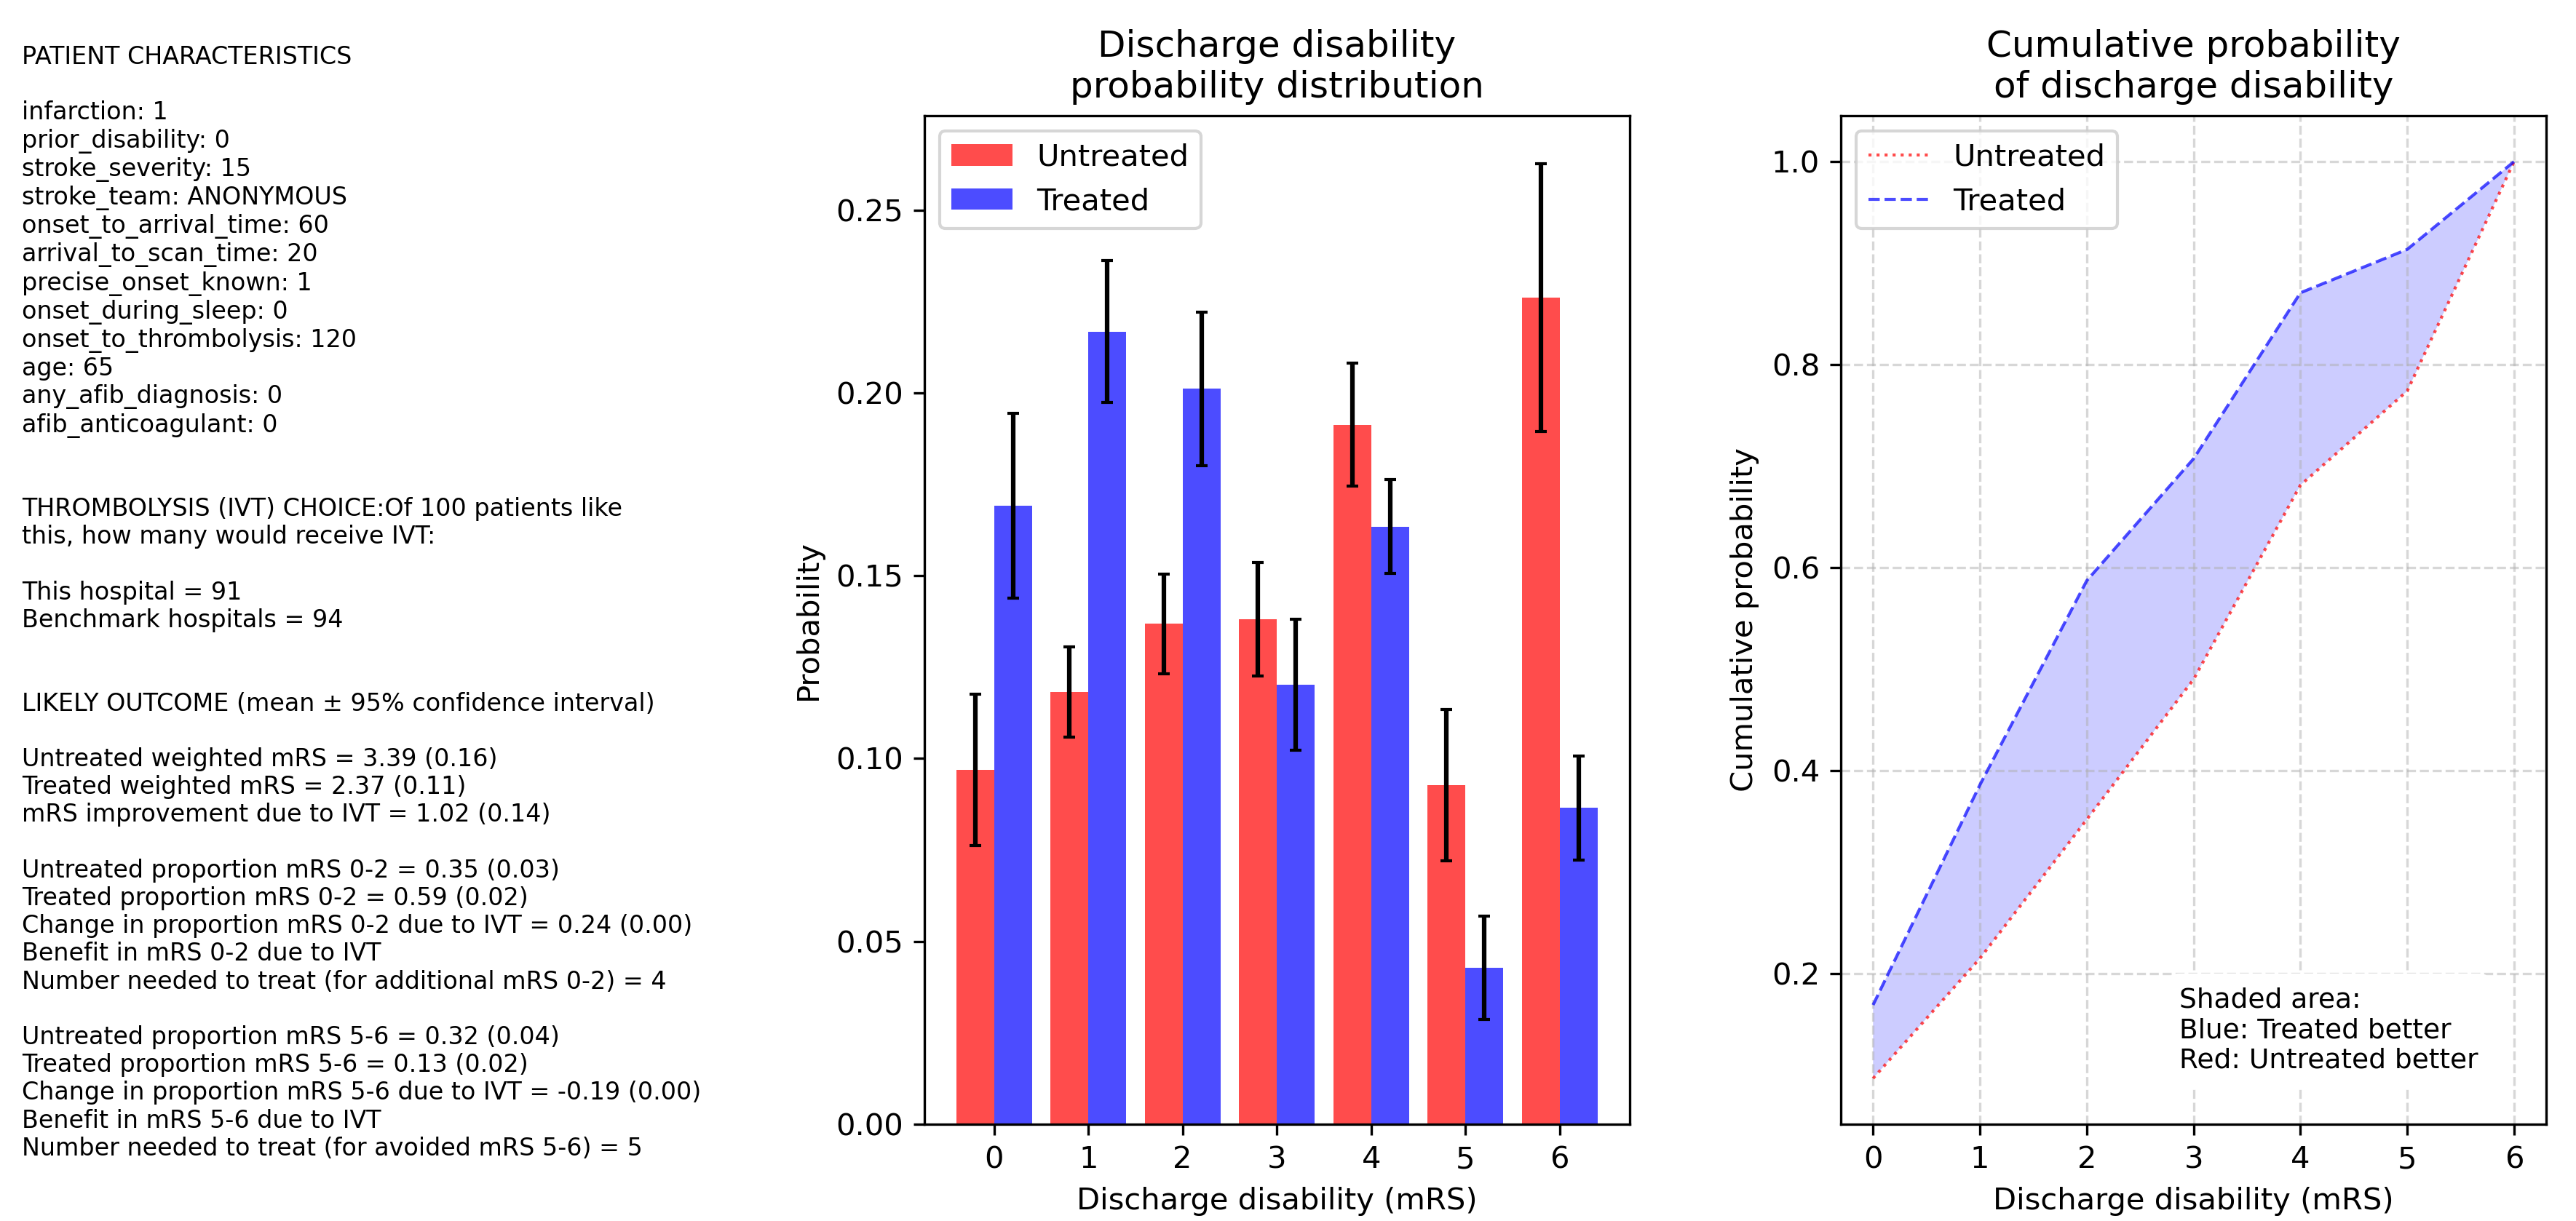
\includegraphics[width=1.0\linewidth]{images/prototype_patient_ideal}
    \caption{Enter Caption}
    \label{fig:example_patient_outcome}
\end{figure}


\begin{figure}
    \centering
    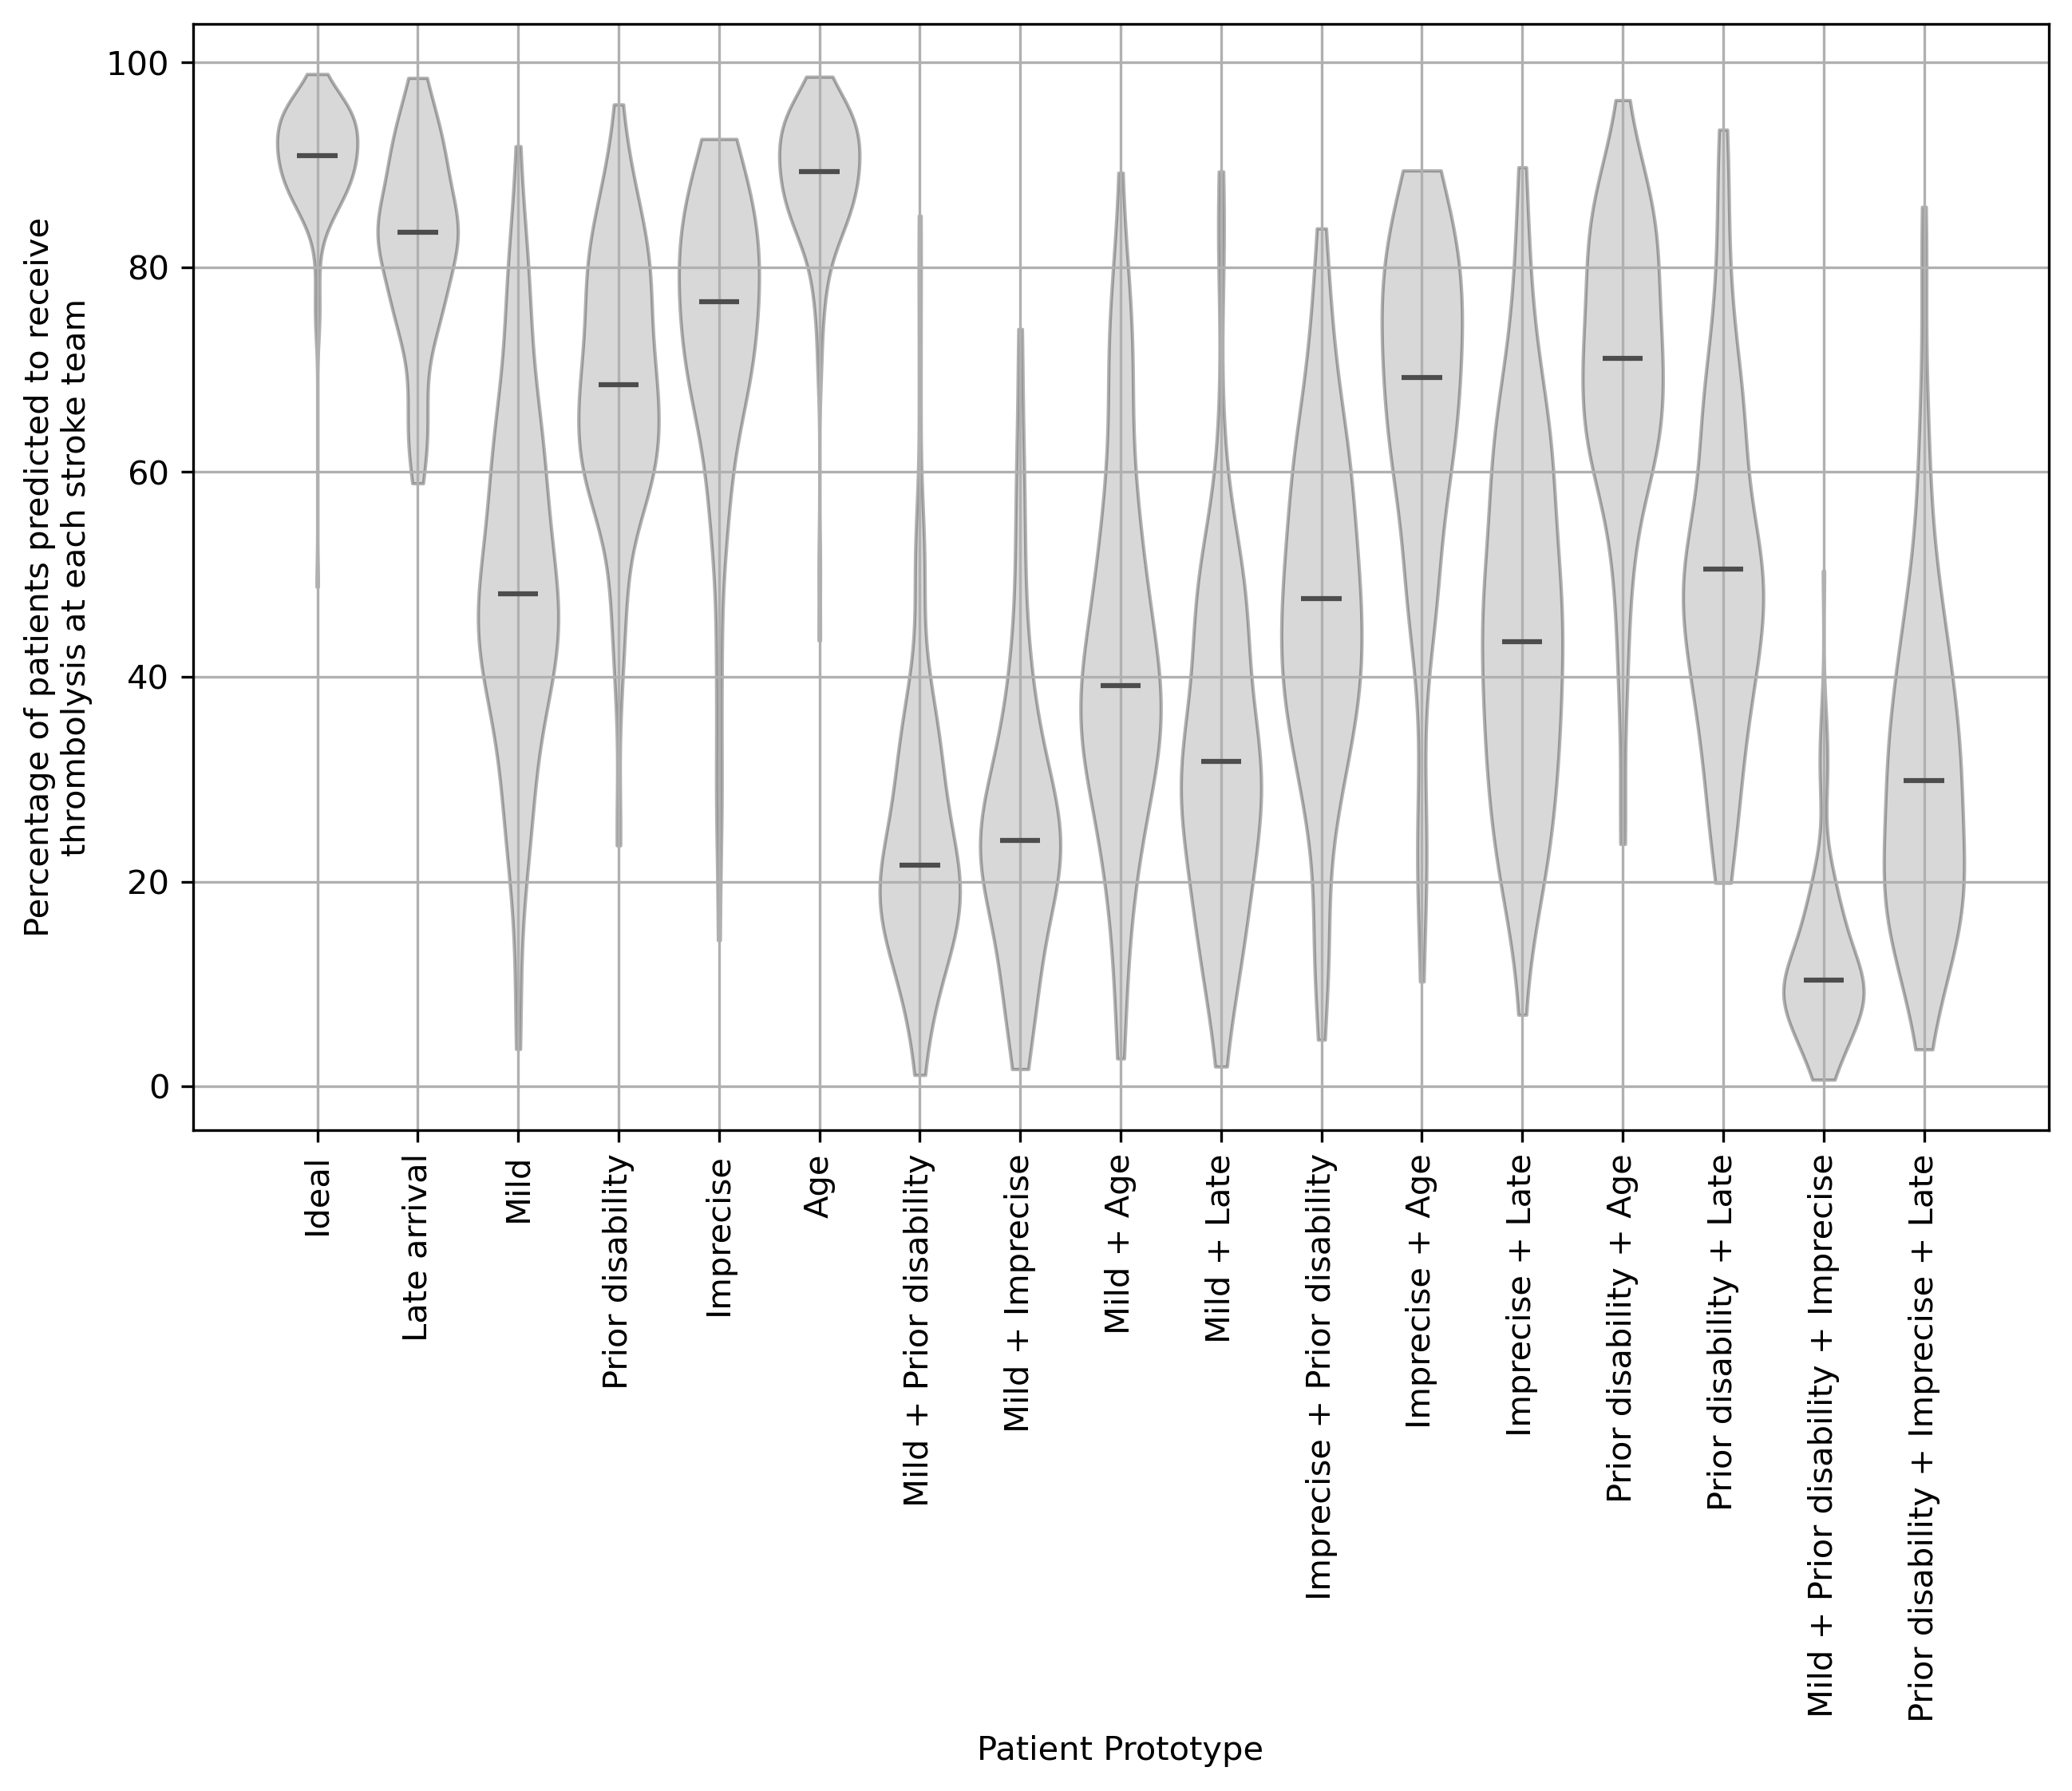
\includegraphics[width=0.75\linewidth]{images/prototype_patients_all_teams}
    \caption{Enter Caption}
    \label{fig:thrombolysis_rates_prototype_patients}
\end{figure}


\begin{minipage}{1\textwidth}
\small
\begin{longtable}{p{5cm}| p{1.5cm} p{1.5cm} p{1.5cm}| p{1.5cm} p{1.5cm} p{1.5cm}}
\caption{Predicted outcomes for patient prototypes. \textit{Ideal}: Onset-to-arrival = 90 minutes; arrival-to-scan = 15 minutes; onset-to-thrombolysis = 120 minutes; stroke severity (NIHSS) = 15; pre-stroke disability (mRS) = 0; age = 72.5; Precisely known onset; onset not during sleep; stroke type = Infarction; patient has no atrial fibrillation and is not receiving anticoagulants for atrial fibrillation. \textit{Late arrival}: as \textit{ideal} but onset-to-arrival = 225 minutes and onset-to-thrombolysis = 255 minutes. \textit{Mild}; As \textit{ideal} but stroke severity = 3; \textit{Prior disability}: as \textit{ideal} but pre-stroke disability = 3; \textit{Imprecise}: as \textit{ideal} but stroke onset time estimated. \textit{Age}: as \textit{ideal} but age = 87.5. Results show probability-weighted disaibility at discharge, and the proportion of patients predicted to have a very poor outcome (mRS 5-6).}\\
\toprule
\endhead
Patient prototype & Untreated probability-weighted mRS & Treated probability-weighted mRS & Improve-ment & Untreated proportion mRS 5-6 & Treated proportion mRS 5-6 & Improve-ment\tabularnewline
\midrule
Ideal & 3.21 & 2.42 & 0.79 & 0.29 & 0.14 & 0.15\tabularnewline
Late & 3.21 & 2.88 & 0.34 & 0.29 & 0.14 & 0.15\tabularnewline
Mild & 1.23 & 1.20 & 0.03 & 0.02 & 0.02 & 0.00\tabularnewline
Prior disability & 4.33 & 3.73 & 0.60 & 0.44 & 0.28 & 0.16\tabularnewline
Imprecise & 3.41 & 2.48 & 0.93 & 0.33 & 0.15 & 0.18\tabularnewline
Age & 3.99 & 3.34 & 0.65 & 0.46 & 0.31 & 0.15\tabularnewline
Mild + Prior disability & 2.88 & 2.70 & 0.19 & 0.07 & 0.06 & 0.02\tabularnewline
Mild + Imprecise & 1.33 & 1.27 & 0.06 & 0.03 & 0.02 & 0.01\tabularnewline
Mild + Age & 1.65 & 1.59 & 0.06 & 0.04 & 0.04 & 0.00\tabularnewline
Mild + Late & 1.23 & 1.63 & -0.40 & 0.02 & 0.02 & 0.00\tabularnewline
Imprecise + Prior disability & 4.44 & 3.79 & 0.65 & 0.48 & 0.31 & 0.17\tabularnewline
Imprecise + Age & 4.13 & 3.36 & 0.76 & 0.49 & 0.32 & 0.18\tabularnewline
Imprecise + Late & 3.41 & 2.96 & 0.45 & 0.33 & 0.15 & 0.15\tabularnewline
Prior disability + Age & 4.71 & 4.42 & 0.28 & 0.55 & 0.45 & 0.09\tabularnewline
Prior disability + Late & 4.44 & 3.68 & 0.76 & 0.48 & 0.24 & 0.24\tabularnewline
Mild + Prior disability + Imprecise & 3.04 & 2.76 & 0.27 & 0.12 & 0.09 & 0.03\tabularnewline
Prior disability + Imprecise + Late & 4.44 & 3.68 & 0.76 & 0.48 & 0.24 & 0.24\tabularnewline
\bottomrule
\label{tab:prototype_outcomes}
\end{longtable}
\normalsize
\end{minipage}

Actual use of thrombolysis (35.1\% of 4 hour ischaemic stroke arrivals treated)
(43.2\% of 4 hour ischaemic stroke arrivals treated)


\begin{table}
\small
\caption{Health economic analysis: Analysis for  populations based on predicted benefit (or dis-benefit) of thrombolysis. The analysis compares the populations currently treated, or the population that would be treated using \textit{benchmark} decisions (the majority vote of the predicted choice of the the 25 stroke teams most likely to use thrombolysis). Results are shown for (a) the treated populations, and (b) adjusted for 1,000 emergency stroke admissions }
\label{tab:main}

\begin{subtable}{1\textwidth}
\caption{}
\begin{tabular}{p{2.0cm} p{1.4cm} p{1.3cm} p{1.3cm} p{1.5cm} p{1.3cm} p{1.4cm} p{1.3cm} p{1.3cm} }
\toprule
Population & Group & Death & Survival (median years) & Care years (median) & QALYs & \raggedright Discounted cost per patient & Proportion mRS 0-2 & Proportion mRS 5-6\tabularnewline
\midrule
Actual & Untreated & 17.1\% & 7.60 & 0.28 & 5.020 & £20,370 & 47.1\% & 23.9\%\tabularnewline
& Treated & 14.2\% & 7.91 & 0.25 & 5.258 & £19,806 & 53.9\% & 19.3\%\tabularnewline
& Difference & -2.9\% & 0.31 & -0.03 & 0.238 & -£565 & 6.8\% & -4.7\%\tabularnewline
\midrule
Benchmark & Untreated & 17.4\% & 7.63 & 0.28 & 5.036 & £20,388 & 46.5\% & 24.1\%\tabularnewline
& Treated & 14.4\% & 7.93 & 0.25 & 5.269 & £19,784 & 53.4\% & 19.4\%\tabularnewline
& Difference & -3.0\% & 0.30 & -0.03 & 0.234 & -£603 & 6.9\% & -4.8\%\tabularnewline
\bottomrule
\end{tabular}
\end{subtable}%

\vspace{3mm}

\begin{subtable}{1\textwidth}
\centering
\caption{Analysis for 1,000 emergency stroke admissions (all stroke types)}
\begin{tabular}{p{1.9cm} p{1.9cm} p{1.9cm} p{1.9cm} p{1.9cm} p{1.9cm} p{2.2cm}}
\toprule
Population & Proportion treated & QALYs added & Healthcare costs saved & \raggedright Thrombolysis cost (£450 per patient) & \raggedright Cost per QALY added & \raggedright Net cost of thrombolysis\tabularnewline
\midrule
Actual & 11.0\% & 26.3 & £62,294 & £49,658 & £1,890 & -£12,637\tabularnewline
Benchmark & 13.6\% & 31.7 & £81,914 & £61,117 & £1,927 & -£20,797\tabularnewline
\bottomrule
\end{tabular}
\end{subtable}
\label{tab:health_econ}
\end{table}

\normalsize
